\chapter{Troisi\`eme annexe}
\label{annexe:C}

\section{La surcharge des op\'erateurs}

\paragraph{Programmation paresseuse}

Pour commencer \`a me familiariser avec la diff\'erentiation automatique, j'ai d'abord essay\'e de 
concevoir un programme qui d\'erive en programmation fonctionnelle. D'apr\`es l'article de Karczmarczuk \cite{paresseuse}, il est possible 
de calculer la diff\'erentiation automatique avec un langage fonctionnel de mani\`ere paresseuse.
La s\'emantique du programme original va être \'etendue par surcharge des op\'erateurs en utilisant
les r\`egles usuelles de d\'erivation. Par exemple, la r\`egle de Leibniz $(fg)'=f'g+fg'$ o\`u la r\`egle
d'encha\^inement : $(f(g(x))'=f'(g(x))g(x)$. Pour toutes op\'erations \'el\'ementaires, nous allons surcharger
par les op\'erations de d\'erivation. Pour cela, on consid\`ere une paire $(e,e')$ qui repr\'esente la valeur
orginale et sa d\'eriv\'ee. De cette mani\`ere, les constantes seront repr\'esent\'ees par $(c,0)$ et la variable
$(x,1)$. Toutes les op\'erations vont être surcharg\'ees pour ce type : $(f,f')+(g,g')=(f+g,f'+g')$, 
$(f,f')\cdot(g,g')=(f\cdot g,f'\cdot g+f\cdot g')$, $cos(f,f')=(cos(f),cos(f)\cdot f')$ et ainsi de suite.

Le langage fonctionnel que j'ai choisi est caml. On commence par d\'efinir un type expression qui traduit les op\'erations \'el\'ementaires. Comme il
 s'agit d'un exemple, la liste est non exhaustive. Le type expression est d'abord introduit, il va nous permettre d'analyser le type d'op\'eration.
En caml, il est impossible de faire un "match" sur une fonction par exemple : \begin{verbatim}| cos -> sin \end{verbatim}
c'est pour cette raison que l'on d\'efinit un constructeur de type : expression. 
{\small
\begin{verbatim}
type expression= 
    Const of float
  | Var of string
  | Opp of expression
  | Plus of expression*expression
  | Moins of expression*expression
  | Mult of expression*expression
  | Quot of expression*expression
  | Puiss of expression*float
  | Cos of expression
  | Sin of expression
  | Exp of expression
  | Log of expression
;;
\end{verbatim}
}
\noindent
Pour diff\'erentier nos constantes de nos variables, il faut introduire lors de l'\'evaluation un
environnement qui fournira la valeur de chaque variable. Par exemple si $x=3.5$ et $y=-2.1$,
$env=[("x",3.5);("y",-2.1)]$ (les parenth\`eses ne sont pas n\'ecessaires mais permettent de bien
comprendre qu'il s'agit d'une liste de couples).


Ainsi, pour \'evaluer une expression, nous n'aurons plus qu'\`a faire :

\begin{verbatim}
let rec evaluer env expr = match expr with
    Const c-> c 
  | Var v->(try List.assoc v env with Not_found ->
 raise(Unbound_variable v))
  | Opp f-> -.evaluer env f
  | Plus(f,g) -> evaluer env f +. evaluer env g
  | Moins(f,g) -> evaluer env f -. evaluer env g
  | Mult(f,g) -> evaluer env f *. evaluer env g
  | Quot(f,g) -> evaluer env f /. evaluer env g
  | Puiss(f,g) ->(evaluer env f)**g
  | Cos(f) -> cos(evaluer env f)
  | Sin(f) -> sin(evaluer env f)
  | Log(f) -> log (evaluer env f)
  | Exp(f) ->  exp (evaluer env f)
 ;;
\end{verbatim}
\noindent
{\tt List.assoc v env} permet de renvoyer l'\'el\'ement correspondant \`a {\tt v} dans la liste de couple {\tt env}. Avec notre exemple,
{\tt List.assoc "x" env} retourne {\tt 3.5}. Cette \'evaluation est la traduction du GAO. Le point apr\`es l'op\'erateur signifie que les composantes sont des {\it float}. (Les op\'erateurs
ne sont pas surcharg\'es et le \verb!+! est pour les entiers).


Pour \'evaluer la d\'eriv\'ee: 

{\small
\begin{verbatim}
let rec derive expr dv =
    match expr with
      Const c -> Const 0.0
    | Var v -> if v = dv then Const 1.0 else Const 0.0
    | Opp f -> Opp(derive f dv)
    | Plus(f, g) -> Plus(derive f dv, derive g dv)
    | Moins(f, g) -> Moins(derive f dv, derive g dv)
    | Mult(f, g) -> Plus(Mult(f, derive g dv), Mult(derive f dv, g))
    | Quot(f, g) -> Quot(Moins(Mult(derive f dv, g), Mult(f, derive g dv)),
                         Mult(g, g))
    | Puiss(f,g) -> Mult(Const g,Mult(derive f dv,f))
    | Cos(f) -> Opp(Mult(Sin(f),derive f dv))
    | Sin(f) -> Mult(Cos(f),derive f dv)
    | Exp(f) -> Mult(derive f dv,Exp(f))
    | Log(f) -> Quot(derive f dv,f)
 ;;
\end{verbatim}
}
\noindent
Karczmarczuk a propos\'e une mani\`ere d'obtenir les d\'eriv\'ees d'ordres sup\'erieurs de mani\`ere paresseuse avec Haskell,
un langage fonctionnel. La d\'efinition pr\'ec\'edente est reprise et \'etendue mais sur une liste infinie $f::f'::f''::f^{(3)}\cdots $
repr\'esentant l'expression avec l'ensemble de ses d\'eriv\'ees. 
De la même mani\`ere, les constantes seront repr\'esent\'ees par $c::0::0\cdots$
et la variable $x::1::0::0\cdots$. En notant $f=(f_0::\bar f)$ et $g=(g_0::\bar g)$ o\`u $f_0$, $g_0$ sont
les \'el\'ements en tête de liste et $\bar f$, $\bar g$ sont les listes queues, les op\'erations seront d\'efinies :
$$f+g = (f_0+g_0::\bar f+\bar g)$$
$$f\cdot g = (f_0\cdot g_0::f\cdot \bar g+\bar f\cdot g)$$
$$f/g = w \text{  o\`u  }(f_0/g_0::(\bar f\cdot g+f \cdot\bar g)\cdot w^2)$$


\noindent
On observe que la d\'efinition est auto-r\'ecursive. \'Evidemment, nous ne devrons pas \'evaluer toute la liste mais seulement les 
d\'eriv\'ees qui nous int\'eressent. Si on essaye d'obtenir {\tt w}, on boucle \`a l'infini! 
\'Etant donn\'e que {\it Caml}\footnote{{\url http://caml.inria.fr/}} n'est pas un langage paresseux, contrairement \`a Haskell, il a fallu construire un nouveau type que l'on 
\'evaluera uniquement quand nous en aurons besoin.


{\small
\begin{verbatim}
type 'a glacon =
| Inconnu of (unit -> 'a)
| Connu of ' a;;
\end{verbatim}
}
\noindent
Le type \verb!(unit -> 'a)! repr\'esente une fonction sans argument. Le r\'esutlat n'est que potentiellement pr\'esent; uniquement 
lorsque l'on \'evaluera cette fonction.

{\small
\begin{verbatim}
type 'a liste_paresseuse =
| Nil
| Cons of 'a cellule
and 'a cellule = { hd : 'a; mutable tl : 'a liste_paresseuse glacon};;
\end{verbatim}
}


{\small
\begin{verbatim}
let force cellule =
  let glacon = cellule.tl in
  match glacon with
  | Connu valeur -> valeur
  | Inconnu g ->
     let valeur = g () in
     cellule.tl <- Connu valeur;
     valeur;;
\end{verbatim}
}
\noindent
Forcer la cellule revient \`a \'evaluer la fonction \verb!g!.
\begin{figure}
\caption{Temps d'\'evaluation du gradient en mode direct par surcharge des op\'erateurs sur 
des listes et vecteurs avec caml}
\begin{center}
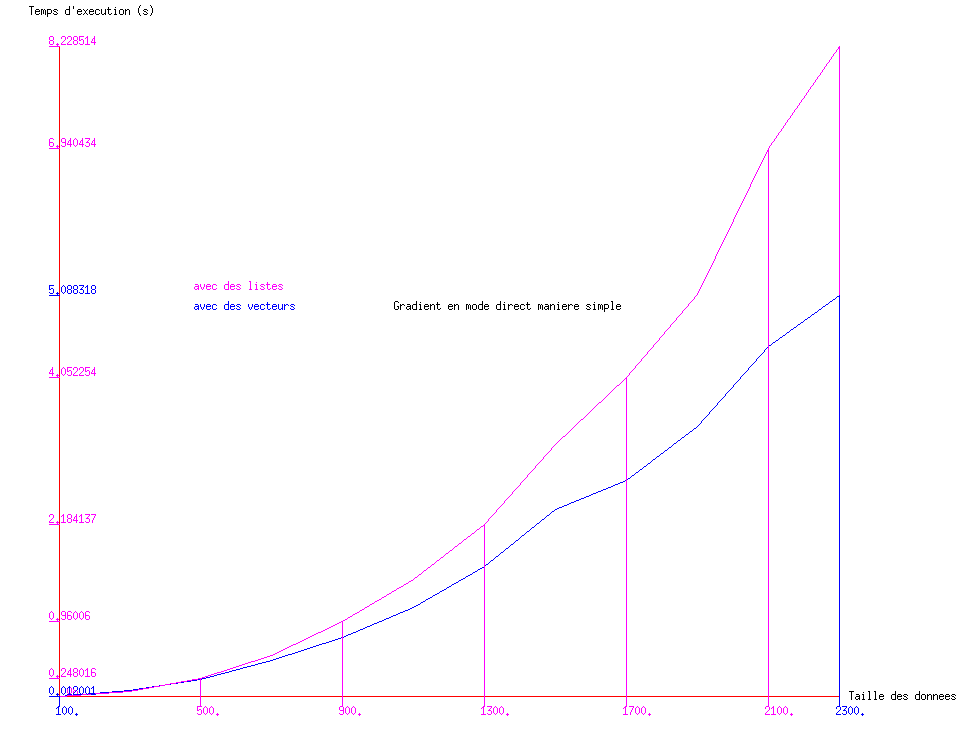
\includegraphics[scale=0.6]{figures/caml1.png}
\end{center}
\label{fig:caml1}
\end{figure}
La figure \ref{fig:caml1} illustre le fait que ces op\'erations impliquent des structures de plus en plus complexes \`a g\'erer.




On peut g\'en\'eraliser les listes infinies \`a plusieurs dimensions avec des d\'eriv\'ees partielles :
$f=(f_0,[\bar f_1,\cdots, \bar f_n] $ o\`u $\bar f_k=(\partial f/\partial f_k,[\cdots \text{ d\'eriv\'ees de }f_k' \cdots])$.
L'inconv\'enient d'une telle m\'ethode vient de la structure qui est rapidement lourde \`a g\'erer; les listes sont tr\`es dures
\`a manipuler lorsqu'elles sont de grandes tailles; $\mathcal{O}(n)$ dans le pire des cas et les vecteurs ne sont pas dynamiques.\\


